\section{Algorytm \textit{RPNI}}
\label{sec:rpni}

Algorytm \textit{RPNI} (\textit{Regular Positive and Negative Inference}) \cite{RPNI} jest jednym z klasycznych algorytmów do odkrywania gramatyki języka regularnego. Dokonuje on generalizacji na podstawie zbiorów przykładów pozytywnych oraz negatywnych, wykorzystując podejście łączenia stanów w akceptorze drzewa prefiksów (PTA).

Model algorytmu zakłada, że język docelowy jest regularny, a dostępne dane (przykłady pozytywne \( S^+ \) i negatywne \( S^- \)) są wystarczająco reprezentatywne, aby umożliwić skonstruowanie minimalnego deterministycznego automatu skończonego (DFA). Proces ten polega na iteracyjnym scalaniu stanów w PTA w celu zbudowania modelu akceptującego wszystkie przykłady pozytywne i odrzucającego negatywne.

\subsection{Metoda}

Algorytm RPNI pozwala na indukcję minimalnego deterministycznego automatu skończonego (DFA), który jest zgodny z danymi pozytywnymi (\( S^+ \)) i danymi negatywnymi (\( S^- \)). Jego działanie opiera się na kilku kluczowych krokach, które prowadzą do iteracyjnego generalizowania języka \( L \) w sposób kontrolowany.

\paragraph*{Opis algorytmu.}
Algorytm RPNI składa się z następujących etapów:
\begin{enumerate}
    \item \textbf{Budowa akceptoru drzewa prefiksów (PTA):}
        Zbiór \( S^+ \) jest używany do budowy automatu reprezentującego dokładnie wszystkie słowa z \( S^+ \). Automatyczny akceptor prefiksów dokładnie reprezentuje język \( L(S^+) \).
    \item \textbf{Iteracyjne łączenie stanów:}
        Algorytm przegląda pary stanów w PTA i sprawdza, czy można je połączyć bez naruszania zgodności z \( S^- \). Połączenie stanów prowadzi do generalizacji języka \( L \).
    \item \textbf{Weryfikacja zgodności z \( S^- \):}
        Dla każdej potencjalnej zmiany algorytm sprawdza, czy żadne słowo z \( S^- \) nie jest akceptowane przez zmodyfikowany automat.
    \item \textbf{Zakończenie:} 
        Algorytm kończy działanie, gdy żadne dodatkowe pary stanów nie mogą być połączone. Wynikowy automat jest minimalny i deterministyczny.
\end{enumerate}

\paragraph*{Zalety algorytmu RPNI:}
\begin{itemize}
    \item \textbf{Minimalizacja DFA:} Wynikowy automat jest zawsze minimalny, zgodny z \( S^+ \) i \( S^- \).
    \item \textbf{Efektywność:} Algorytm działa w czasie wielomianowym względem rozmiaru danych wejściowych.
    \item \textbf{Zbieżność identyfikacji (identification in the limit \cite{GOLD1967447}):} RPNI gwarantuje poprawne działanie dla klas języków regularnych w przypadku wystarczająco dużego zestawu danych.
\end{itemize}

\subsection{Formalizacja}

Celem niniejszej sekcji jest dostarczenie formalnych definicji oraz narzędzi matematycznych niezbędnych do pełnego zrozumienia algorytmu RPNI. W szczególności omówione zostaną kluczowe koncepcje, takie jak deterministyczny automat skończony (DFA) oraz akceptor drzewa prefiksów (Prefix Tree Acceptor, PTA), które stanowią podstawę teoretyczną algorytmu. Formalizacja ta pozwala na przejście od zestawu przykładów pozytywnych i negatywnych do precyzyjnego opisu języków regularnych oraz konstrukcji ich reprezentacji w postaci minimalnych automatów. Ponownie potrzebne nam są: definicja \ref{def:dfa} (DFA), definicja \ref{def:word_acceptance} (akceptowanie słowa) i definicja \ref{def:regular_language} (język regularny).

\begin{definition}[Zbiór pozytywny $S^+$]
    Zbiorem pozytywnym lub zbiorem przykładów pozytywnych nazywamy zbiór takich słów $w$, że \( w \in L \).
\end{definition}

\begin{definition}[Zbiór negatywny $S^-$]
    Zbiorem negatywnym lub zbiorem przykładów negatywnych nazywamy zbiór takich słów $w$, że \( w \notin L \).
\end{definition}

Oczywistą, ale wartą odnotowania implikacją jest to, że zbiór przykładów pozytywnych i zbiór przykładów negatywnych są rozłączne (\( S^+ \cap S^- = \emptyset \)).

\begin{definition}[Akceptor drzewa prefiksów (Prefix Tree Acceptor, PTA)]  
    \label{def:pta}
    Dla zbioru \( S^+ \), akceptor drzewa prefiksów \( PTA(S^+) \) to deterministyczny automat skończony \( M = (Q, \Sigma, \delta, q_0, F) \), gdzie:
    \begin{itemize}
        \item \( Q \): zbiór wszystkich prefiksów słów z \( S^+ \),
        \item \( \Sigma \): alfabet słów w \( S^+ \),
        \item \( \delta(q, a) = qa \): przejście w drzewie jest zdefiniowane przez konkatenację z symbolem \( a \),
        \item \( q_0 = \epsilon \): stan początkowy reprezentuje pusty prefiks,
        \item \( F = \{q \in Q \mid q \text{ jest pełnym słowem w } S^+\}\).
    \end{itemize}
\end{definition}

\begin{definition}[Łączenie stanów]
    \label{def:state_merging}
    Łączenie dwóch stanów \( q_1, q_2 \in Q \) w deterministycznym automacie skończonym \( M = (Q, \Sigma, \delta, q_0, F) \) polega na utworzeniu nowego automatu \( M' = (Q', \Sigma, \delta', q_0', F') \), gdzie zbiór stanów po łączeniu zawiera \( q_1 \) jako reprezentanta obu stanów, a \( q_2 \) jest usunięty. Ponadto funkcja przejścia jest odpowiednio zaktualizowana, aby przekierować wszystkie przejścia z \( q_2 \) na \( q_1 \). Jeśli \( q_2 \) był stanem akceptującym, \( q_1 \) również staje się stanem akceptującym.
    \begin{itemize}
        \item \( Q' = Q \setminus \{q_2\} \),
        \item \( \delta'(q, a) = 
        \begin{cases} 
            q_1 & \text{jeśli} \space \delta(q, a) = q_2, \\
            \delta(q, a) & \text{w przeciwnym przypadku,}
        \end{cases}
        \),
        \item \( F' =
        \begin{cases} 
            F & \text{jeśli } q_2 \notin F \\
            F \setminus \{q_2\} & \text{jeśli } q_2 \in F \land q_1 \in F \\
            (F \setminus \{q_2\}) \cup \{q_1\} & \text{jeśli } q_2 \in F \land q_1 \notin F \\
        \end{cases}
        \).
    \end{itemize}
\end{definition}

\paragraph*{Formalny proces algorytmu RPNI.}
\begin{itemize}
    \item \textbf{Konstrukcja \( PTA(S^+) \):} Utwórz akceptor drzewa prefiksów na podstawie \( S^+ \).
    \item \textbf{Iteracyjne łączenie stanów:} 
    \begin{itemize}
        \item Sprawdzaj każdą parę stanów \( q_1, q_2 \in Q \) w \( PTA(S^+) \).
        \item Połącz stany zgodnie z definicją \ref{def:state_merging}.
    \end{itemize}
    \item \textbf{Zakończenie:} Proces kończy się, gdy żadne kolejne łączenie stanów nie jest możliwe.
\end{itemize}

\paragraph*{Wynik:}
Rezultatem algorytmu jest minimalny DFA \( M \), który akceptuje wszystkie słowa z \( S^+ \) i żadne słowo z \( S^- \). Dzięki iteracyjnemu łączeniu stanów \( PTA(S^+) \) zostaje stopniowo uproszczony do ostatecznej postaci minimalnego automatu.

\subsection{Złożoność}

Algorytm \textit{RPNI} charakteryzuje się złożonością wielomianową względem rozmiaru danych wejściowych. Aby dokładnie określić jego złożoność czasową i pamięciową, należy zdefiniować kluczowe parametry:
\begin{itemize}
    \item \(|S^+|\) - liczba słów w zbiorze pozytywnych przykładów,
    \item \( l^+ \) - maksymalna długość słowa w \( S^+ \),
    \item \(|S^-|\) - liczba słów w zbiorze negatywnych przykładów,
    \item \( l^- \) - maksymalna długość słowa w \( S^- \),
    \item \(|\Sigma|\) - rozmiar alfabetu.
\end{itemize}

\paragraph*{Złożoność czasowa}
Algorytm RPNI składa się z dwóch głównych etapów:
\begin{enumerate}
    \item \textbf{Konstrukcja drzewa prefiksowego (PTA):}
    Utworzenie PTA wymaga przejścia przez wszystkie słowa w \( S^+ \), co ma złożoność \( O(|S^+| \cdot l^+) \).
    \item \textbf{Iteracyjne łączenie stanów:}
    Liczba stanów w \( PTA(S^+) \) jest równa liczbie wszystkich prefiksów słów w \( S^+ \), co w najgorszym przypadku wynosi \( O(|S^+| \cdot l^+) \). Każde łączenie dwóch stanów wymaga sprawdzenia, czy wynikowy automat jest zgodny z danymi negatywnymi \( S^- \). Sprawdzenie tego wymaga przejścia przez \( |S^-| \) słów. Etap ten ma, więc złożoność \( O((|S^+| \cdot l)^2 \cdot |S^-|) \).
\end{enumerate}

Łączna złożoność czasowa algorytmu wynosi:
\[
O(|S^+| \cdot l^+ + (|S^+| \cdot l^+)^2 \cdot |S^-|),
\]
co można uprościć do:
\[
O((|S^+| \cdot l^+)^2 \cdot |S^-|).
\]


\paragraph*{Złożoność pamięciowa}
Algorytm przechowuje następujące struktury danych:
\begin{itemize}
    \item \textbf{Drzewo prefiksowe (PTA):}  
    PTA zawiera \( O(|S^+| \cdot l^+) \) stanów, z których każdy może mieć do \( |\Sigma| \) przejść. Wymagana pamięć wynosi:
    \[
    O(|S^+| \cdot l^+ \cdot |\Sigma|).
    \]

    \item \textbf{Negatywne przykłady (\( S^- \)):}  
    Przechowywane są do weryfikacji zgodności połączeń. Przechowywanie \( |S^-| \) słów o maksymalnej długości \( l^- \) wymaga:
    \[
    O(|S^-| \cdot l^-).
    \]
\end{itemize}

Łączna złożoność pamięciowa algorytmu wynosi:
\[
O(|S^+| \cdot l^+ \cdot |\Sigma| + |S^-| \cdot l^-).
\]

\paragraph*{Czynniki wpływające na złożoność}
Główne elementy mające wpływ na wydajność algorytmu RPNI to:
\begin{itemize}
    \item \textbf{Rozmiar zbioru pozytywnych przykładów (\( S^+ \)):} Większy zbiór przykładów pozytywnych prowadzi do większego drzewa prefiksowego oraz większej liczby stanów do połączenia.
    \item \textbf{Rozmiar zbioru negatywnych przykładów (\( S^- \)):} Większy zbiór przykładów negatywnych zwiększa liczbę weryfikacji podczas łączenia stanów.
    \item \textbf{Długość słów ($l^+$ i $l^-$):} Dłuższe słowa zwiększają zarówno liczbę stanów w \( PTA \), jak i czas przetwarzania weryfikacji.
    \item \textbf{Rozmiar alfabetu (\( |\Sigma| \)):} Większy alfabet zwiększa liczbę przejść w \( PTA \).
\end{itemize}

\subsection{Przykład działania}

Poniżej przedstawiono krok po kroku przykład działania algorytmu RPNI. Rozważmy język $L$, który składa się ze słów zawierających literę $a$: 
\[
L = \{ w \in \{a, b, c\}^*a\{a, b, c\}^* \},
\]
oraz przyjmijmy następujące zbiory zdań pozytywnych i negatywnych:
\[
S^+ = \{ a, aa, ab, ba, aba, aab, baa, abaaa, baaaa, ac \},
\]
\[
S^- = \{ \epsilon, b, bb, c, bc, bbb, bbbc \}.
\]

Na początku algorytm konstruuje akceptor drzewa prefiksów PTA na podstawie zbioru \( S^+ \). Struktura PTA jest zaprezentowana na rysunku \ref{fig:pta00}. Następnie algorytm iteracyjnie łączy stany w taki sposób, aby zachować zgodność zarówno z danymi negatywnymi (\( S^- \)). 

Warto podkreślić, że kolejność wykonywanych operacji łączenia zależy od konkretnej implementacji algorytmu. Istotne jednak jest to, że niezależnie od przyjętej kolejności wynik końcowy pozostaje taki sam. Dla celów ilustracyjnych stany do połączenia będą wybierane przez autora.

W pierwszej iteracji rozważamy połączenie stanów \( q_0 \) i \( q_1 \). Próba ich scalania nie może zakończyć się powodzeniem, ponieważ naruszyłaby zgodność z danymi negatywnymi (\( S^- \)). Przykładem takiego naruszenia jest słowo \( \epsilon \), które po połączeniu \( q_0 \) i \( q_1 \) zostałoby niesłusznie zaakceptowane. 

W kolejnej iteracji analizujemy stany \( q_1 \) i \( q_2 \). Ich połączenie jest możliwe, ponieważ nie narusza zgodności z danymi negatywnymi (\( S^- \)). W wyniku tej operacji scalania powstaje zaktualizowany graf, przedstawiony na rysunku \ref{fig:pta01}.

\begin{figure}[ht]
    \centering
    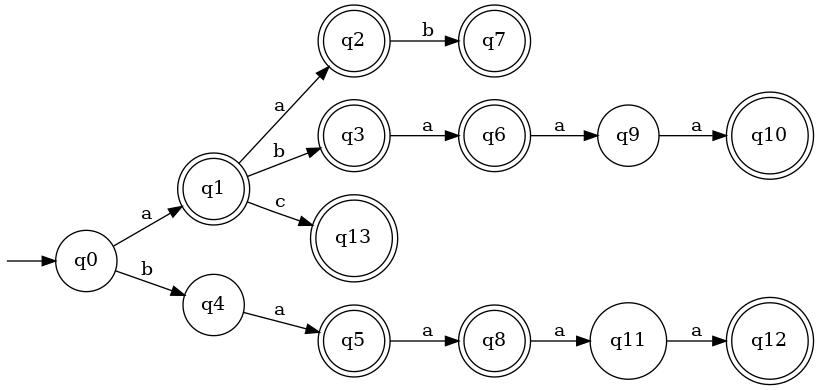
\includegraphics[width=0.8\textwidth]{images/run_example/rpni/0.png}
    \caption{Drzewo prefiksowe (PTA) skonstruowane dla \( S^+ \).}
    \label{fig:pta00}
\end{figure}

\begin{figure}[ht]
    \centering
    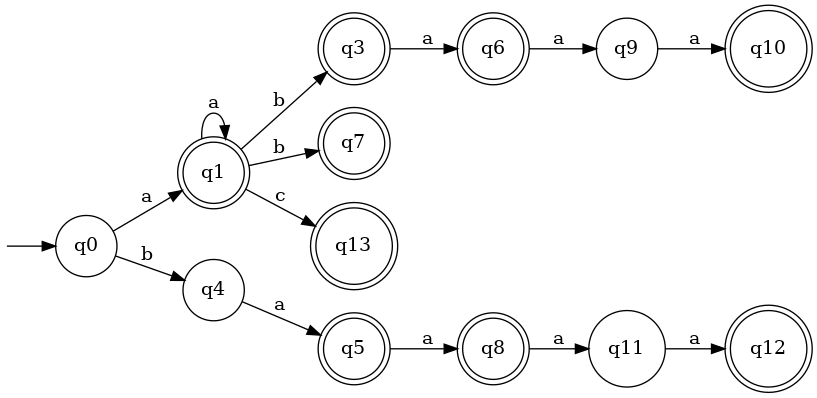
\includegraphics[width=0.8\textwidth]{images/run_example/rpni/1.png}
    \caption{Połączenie stanów \( q1 \) i \( q2 \).}
    \label{fig:pta01}
\end{figure} 

Następne pary stanów będą tak wyznaczane, aby były to poprawne łączenia w celu usprawnienia pokazywania przykładu. Kolejnym krokiem jest połączenie stanów \( q_3 \) i \( q_7 \), co przedstawiono na rysunku \ref{fig:pta02}. Algorytm następnie łączy stany \( q_3 \) i \( q_{13} \), co przedstawiono na rysunku \ref{fig:pta03}. Połączenie stanów \( q_3 \) i \( q_5 \) prowadzi do zaktualizowanego grafu widocznego na rysunku \ref{fig:pta04}. 

W tym momencie łatwo można zauważyć podobieństwo dwóch gałęzi wychodzących z węzła \( q_3 \). Stąd, w tym kroku algorytm łączy pary stanów: \( q_6 \) i \( q_8 \), \( q_9 \) i \( q_{11} \), oraz \( q_{10} \) i \( q_{12} \). Zaktualizowany graf przedstawiono na rysunku \ref{fig:pta05}. 

Następnie zostaje przeprowadzone łączenie stanów \( q_9 \) i \( q_{10} \), \( q_6 \) i \( q_9 \), oraz \( q_3 \) i \( q_6 \). Warte odnotowania jest to, że po raz pierwszy łączymy stan akceptujący z nieakceptującym. W takim przypadku nowy stan będzie akceptujący. Jest to generalizacja, która jest poprawna, ponieważ zawsze sprawdzamy zgodność ze zbiorem \( S^- \).

\begin{figure}[ht]
    \centering
    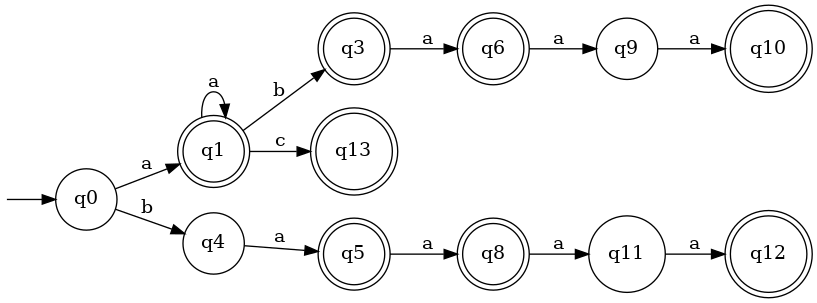
\includegraphics[width=0.8\textwidth]{images/run_example/rpni/2.png}
    \caption{Połączenie stanów \( q3 \) i \( q7 \).}
    \label{fig:pta02}
\end{figure}

\begin{figure}[ht]
    \centering
    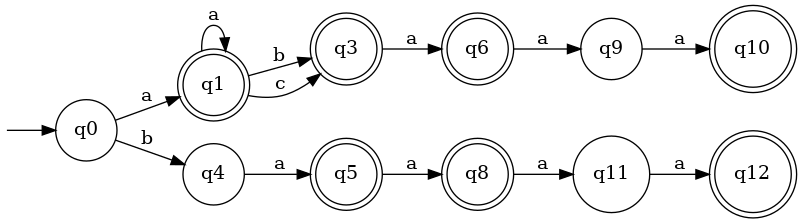
\includegraphics[width=0.8\textwidth]{images/run_example/rpni/3.png}
    \caption{Połączenie stanów \( q3 \) i \( q13 \).}
    \label{fig:pta03}
\end{figure}

\begin{figure}[ht]
    \centering
    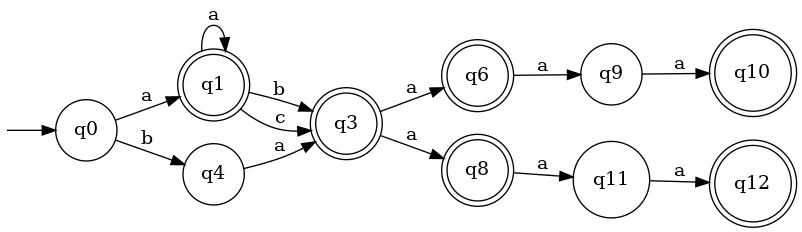
\includegraphics[width=0.8\textwidth]{images/run_example/rpni/4.png}
    \caption{Połączenie stanów \( q3 \) i \( q5 \).}
    \label{fig:pta04}
\end{figure}

\begin{figure}[ht]
    \centering
    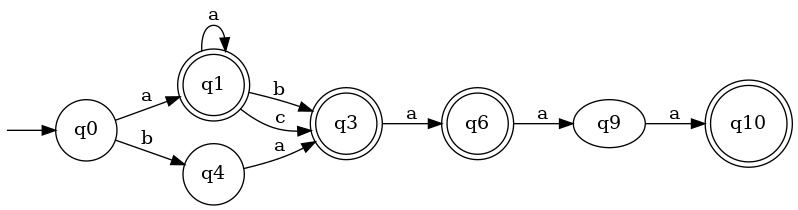
\includegraphics[width=0.8\textwidth]{images/run_example/rpni/5.png}
    \caption{Połączenie stanów \( q6 \) i \( q8 \), \( q9 \) i \( q11 \), oraz \( q10 \) i \( q12 \).}
    \label{fig:pta05}
\end{figure}

Algorytm wykonuje kolejne połączenia stanów, co prowadzi do grafu widocznego na rysunku \ref{fig:pta06}. W tym kroku stany \( q_0 \) i \( q_4 \) zostają połączone. Wynik przedstawiono na rysunku \ref{fig:pta07}. W ostatnim kroku algorytm łączy stany \( q_1 \) i \( q_3 \), uzyskując finalny graf przedstawiony na rysunku \ref{fig:pta08}. 

Nie jest to jednak koniec, ponieważ brakuje przejścia \( c \) ze stanu \( q_0 \). W takim wypadku konieczne jest dodanie nowego cyklicznego przejścia, czyli z \( q_0 \) do \( q_0 \). Po tej operacji uzyskujemy wynikowy DFA, który generuje język \( L \).

\begin{figure}[ht]
    \centering
    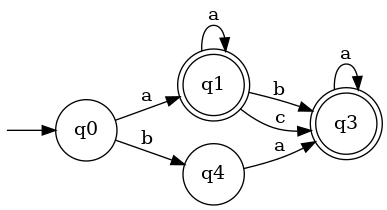
\includegraphics[width=0.4\textwidth]{images/run_example/rpni/6.png}
    \caption{Połączenie stanów \( q9 \) i \( q10 \), \( q6 \) i \( q9 \), oraz \( q3 \) i \( q6 \).}
    \label{fig:pta06}
\end{figure}

\begin{figure}[ht]
    \centering
    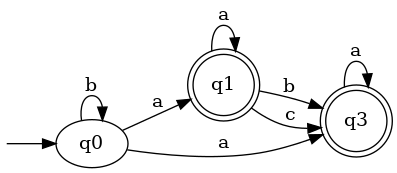
\includegraphics[width=0.4\textwidth]{images/run_example/rpni/7.png}
    \caption{Połączenie stanów \( q0 \) i \( q4 \).}
    \label{fig:pta07}
\end{figure}

\begin{figure}[ht]
    \centering
    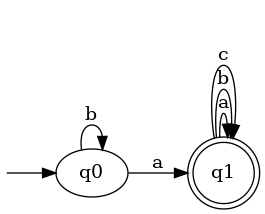
\includegraphics[width=0.4\textwidth]{images/run_example/rpni/8.png}
    \caption{Finalny graf po połączeniu stanów \( q1 \) i \( q3 \).}
    \label{fig:pta08}
\end{figure}
